
\documentclass[12pt]{article}

% Layout.
\usepackage[top=1.0in, bottom=0.75in, left=1in, right=1in, headheight=1.0in, headsep=0pt]{geometry}

% Fonts.
\usepackage{mathptmx}
\usepackage[scaled=0.86]{helvet}
\renewcommand{\emph}[1]{\textsf{\textbf{#1}}}

% TiKZ.
\usepackage{tikz, pgfplots}
\usetikzlibrary{calc}
%\pgfplotsset{my style/.append style={axis x line=middle, axis y line=middle, xlabel={$x$}, ylabel={$y$}, axis equal }}
\pgfplotsset{my style/.append style={axis x line=middle, axis y line=middle, xlabel={$x$}, ylabel={$y$}}}

% Misc packages.
\usepackage{amsmath,amssymb,latexsym}
\usepackage{graphicx}
\usepackage{array}
\usepackage{xcolor}
\usepackage{multicol}

% Commands to set various header/footer components.
\makeatletter
\def\doctitle#1{\gdef\@doctitle{#1}}
\doctitle{Use {\tt\textbackslash doctitle\{MY LABEL\}}.}
\def\docdate#1{\gdef\@docdate{#1}}
\docdate{Use {\tt\textbackslash docdate\{MY DATE\}}.}
\def\doccourse#1{\gdef\@doccourse{#1}}
\let\@doccourse\@empty
\def\docscoring#1{\gdef\@docscoring{#1}}
\let\@docscoring\@empty
\def\docversion#1{\gdef\@docversion{#1}}
\let\@docversion\@empty
\makeatother

% Headers and footers layout.
\makeatletter
\usepackage{fancyhdr}
\pagestyle{fancy}
\fancyhf{} % Clears all headers/footers.
\lhead{\emph{\@doctitle\hfill\@docdate}
\ifnum \value{page} > 1\relax\else\\
\emph{Name: \rule{3.5in}{1pt}\hfill \@docscoring}
\\
\emph{Circle one: \quad Faudree (F01) \hskip 1ex\rule{1pt}{9pt}\hskip 1ex Bueler (F02) \hskip 1ex\rule{1pt}{9pt}\hskip 1ex VanSpronsen (UX1)}
\fi}

\rfoot{\emph{\@docversion}}
\lfoot{\emph{\@doccourse}}
\cfoot{\emph{\thepage}}
\renewcommand{\headrulewidth}{0pt}%
\makeatother

% Paragraph spacing
\parindent 0pt
\parskip 6pt plus 1pt

% A problem is a section-like command. Use \problem{5} to
% start a problem worth 5 points.
\newcounter{probcount}
\newcounter{subprobcount}
\setcounter{probcount}{0}
\newcommand{\problem}[1]{%
\par
\addvspace{4pt}%
\setcounter{subprobcount}{0}%
\stepcounter{probcount}%
\makebox[0pt][r]{\emph{\arabic{probcount}.}\hskip1ex}\emph{[#1 points]}\hskip1ex}
\newcommand{\thesubproblem}{\emph{\alph{subprobcount}.}}

% Subproblems are an enumerate-like environment with a consistent
% numbering scheme. 
% Use \begin{subproblems}\item...\item...\end{subproblems}
\newenvironment{subproblems}{%
\begin{enumerate}%
\setcounter{enumi}{\value{subprobcount}}%
\renewcommand{\theenumi}{\emph{\alph{enumi}}}}%
{\setcounter{subprobcount}{\value{enumi}}\end{enumerate}}

% Blanks for answers in normal and math mode.
\newcommand{\blank}[1]{\rule{#1}{0.75pt}}
\newcommand{\mblank}[1]{\underline{\hspace{#1}}}
\def\emptybox(#1,#2){\framebox{\parbox[c][#2]{#1}{\rule{0pt}{0pt}}}}

% Misc.
\renewcommand{\d}{\displaystyle}
\newcommand{\ds}{\displaystyle}
\def\bc{\begin{center}}
\def\ec{\end{center}}


\doctitle{Math 251: Quiz 9}
\docdate{April 14, 2020}
\doccourse{UAF Calculus I}
\docversion{v-1}
\docscoring{{\Large \strut}\blank{0.8in} / 25}

\begin{document}
25 points possible.  \textcolor{red}{\textbf{No aids (internet, other students, book, calculator, etc.) are permitted.} } You do not need to simplify final answers, but \textcolor{red}{\textbf{answers without supporting work will lose points for completeness and effort.}}

% compare 5.2 #33 which is on webassign
\problem{6} The graph of $f$ is shown.  Evaluate each integral by interpreting it in terms of areas.
\begin{center}
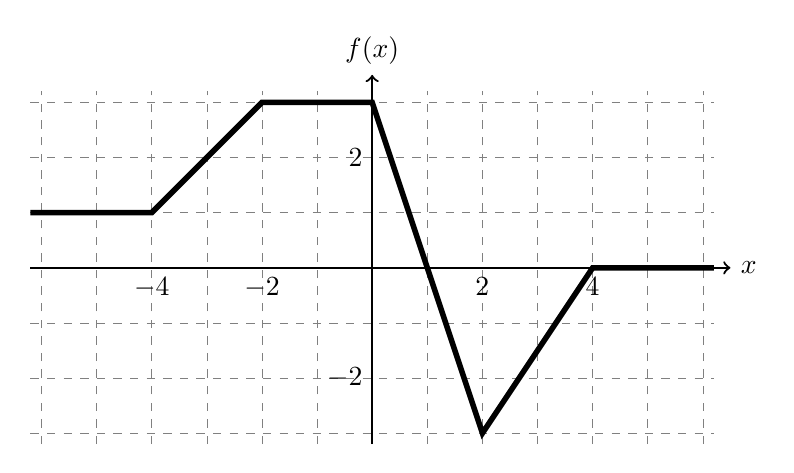
\begin{tikzpicture}[scale=0.7]
\draw [help lines,dashed] (-6.2,-3.2) grid (6.2,3.2);

% axes with labels
\draw [thick, ->] (-6.2,0)--(6.5,0) node[right] {$x$};
\draw [thick, ->] (0,-3.2)--(0,3.5) node[above]{$f(x)$};
\foreach \i in {-4,-2,2,4}
{	\node[below] at (\i,0) {$\i$};
}
\foreach \i in {-2,2}
{	\node[left] at (0,\i) {$\i$};
}

% actual graph
\draw[line width=2pt] (-6.2,1)--(-4,1)--(-2,3)--(0,3)--(2,-3)--(4,0)--(6.2,0);
\end{tikzpicture}
\end{center}

\medskip
\begin{subproblems}
\item $\ds \int_{-4}^{0} f(x)\,dx=$

\medskip
\item $\ds \int_{0}^4 f(x)\,dx=$

\medskip
\item $\ds \int_{4}^{-2} f(x)\,dx=$
\end{subproblems}
\bigskip

% compare 4.9 #63, which is on webassign
\problem{6}  A particle is moving with the given acceleration $a(t)$ and other data.  Find the position $s(t)$ of the particle.
    $$a(t) =  \sin t + \cos t, \quad s(0)=3, \quad v(0)=4 \hspace{80mm}$$
\vfill

\newpage
% compare 5.2 #2
\problem{8}  Consider the graph of $\ds f(x) = 1 + x^2$ below.

\begin{center}
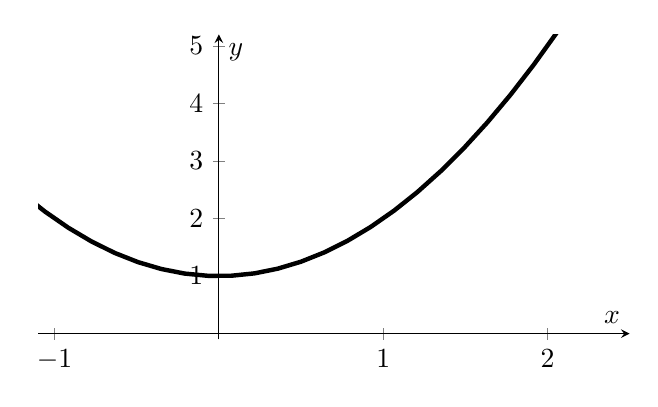
\begin{tikzpicture}
\begin{axis}[scale=1.0, my style, xtick={-1,...,2}, ytick={0,1,2, 3, 4, 5},
xmin=-1.1, xmax=2.5, ymin=-0.1, ymax=5.2, mark size=3.0pt, width=0.75\textwidth, height=0.45\textwidth]
\addplot[domain=-1.2:2.2, ultra thick] {1+x^2};
%\addplot[mark=*,fill=white,only marks] coordinates {(2,1)(5,4)};
\end{axis}
\end{tikzpicture}
\end{center}

\begin{subproblems}
% version 2 will have right endpoints
\item In the figure above, sketch three rectangles corresponding to the $n=3$ Riemann sum on the interval $-1\le x \le 2$.  Use right endpoints.

\medskip
\item Compute the numerical value of the Riemann sum illustrated in part \textbf{a}.  Express your answer as an integer.

\vspace{1.5in}
\item Is your numerical value in part \textbf{b} an overestimate or an underestimate of $\displaystyle \int_{-1}^2 1 + x^2\,dx$?

\vspace{0.3in}
\end{subproblems}

\problem{5} Evaluate the integral by interpreting it in terms of areas: $$\int_{-2}^3 |\tfrac{1}{2} x|\,dx$$ 
\vfill

%\problem{5} Use the properties of the definite integral to find the given integral, given that $\displaystyle \int_a^b f(x)\,dx = 3$ and $\displaystyle \int_a^b g(x)\,dx = -5$

 %	$$\int_a^b \left( 4f(x)+ \dfrac{g(x)}{10} \right)\,dx$$
	
% compare 5.2 #9 which is on WebAssign
%\problem{5}  Use the Midpoint Rule with $n=2$ subintervals to approximate the integral.  Express your answer as a single fraction.
%    $$\int_0^4 x\, 2^{-x}\,dx \approx \hspace{130mm}$$
\vfill

\end{document}